\chapter{はじめに}
\label{chap:00-preface}

このたびは、「やる夫で学ぶ{-}Redux{-} Redux Toolkitは簡単だお・・・」を、手にしていただき誠にありがとうございます。

\begin{reviewimage}%%greetings
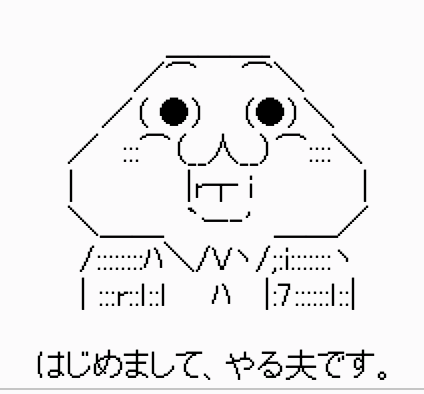
\includegraphics[width=1.0\maxwidth]{./images/00-preface/greetings.png}%
\label{image:00-preface:greetings}
\end{reviewimage}
\vspace*{\baselineskip}
\vspace*{\baselineskip}

私は15年近くVisual Studio上でC\#を使ってUIのあるプログラムを書いていました。
最近は、同一コードでマルチプラットフォーム上で動作するアプリケーションの構築は幾通りもの方法がありますが、
以前は、方法が限られていました。

\vspace*{\baselineskip}

あるとき、あるプロジェクトでは、「Windows、Mac上にて同一UIで動作」が要求されました。
そのために選択したのが、ブラウザ上で動作するWebアプリケーションです。

\vspace*{\baselineskip}

さらに、Webアプリケーションではローカルファイルにアクセスできないため、Electronを使用することで、
Webアプリケーションをマルチプラットフォームで動作するアプリケーションにしました。

\vspace*{\baselineskip}

当時は、WebアプリケーションのフレームワークとしてAngularとReactが候補に挙がりましたが、
Reactの方が学習コストが低いと言われていたため、Reactを学びました。

学習コストが低いとはいえ、壁にブチ当たると時間をかけて調べることを繰り返しました。

\begin{reviewimage}[H]%%greetings02
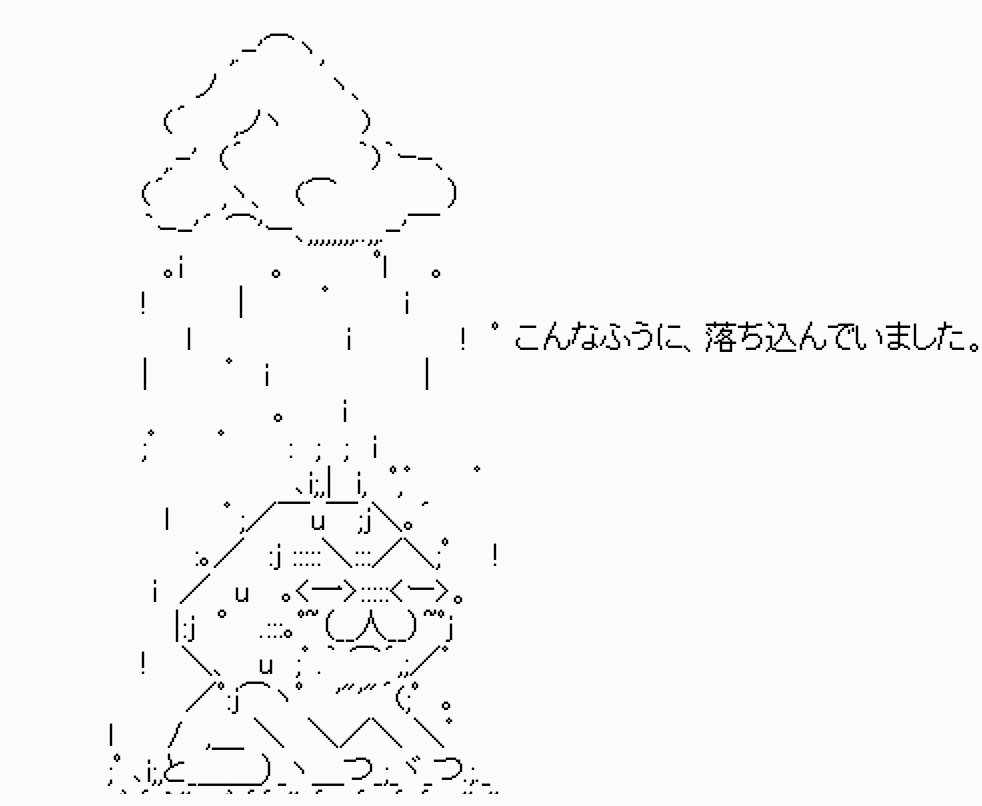
\includegraphics[width=0.7\maxwidth]{./images/00-preface/greetings02.png}%
\label{image:00-preface:greetings02}
\end{reviewimage}
\vspace*{\baselineskip}

本書は、私がReactやReduxを使い始めたときに「こんな本があれば良かったのに・・・」を目指して書きました。
React,Reduxの初学者から中級の方のお役に立てれば幸いです。

\vspace*{\baselineskip}

React、Reduxの解説書やチュートリアルは、書籍・インターネット上にたくさんあります。
しかし、つぎつぎと新機能が追加され本家以外の情報は、あっという間に古くなってしまいます。
この書籍は、掲載情報を最新にするために電子書籍のみとし、古くなった情報は随時更新していきたいと思っています。

\begin{reviewimage}[H]%%greetings03

\includegraphics[width=0.7\maxwidth]{./images/00-preface/greetings03.png}%
\label{image:00-preface:greetings03}
\end{reviewimage}

お気付き点がございましたら、Guthub上へお寄せください。

\vspace*{\baselineskip}

本書は、フロントエンド開発で使用されている

\begin{starteritemize}
\item react
\item redux(redux{-}toolkit)
\end{starteritemize}

を習得するために、開発環境の作成(つまりゼロ)から始め、読書日記アプリケーションを作成します。

\vspace*{\baselineskip}

すでに開発環境を整えている方は、第1章、第2章を飛ばしてもかまいません。

\vspace*{\baselineskip}

また、ゼロからの環境構築、サンプルアプリケーションはGutHubに公開していますが、こちらも最新の情報に更新していくつもりです。
GutHubでは、章毎に別ブランチにしてありますので、写経がメンドウな方は章に対応したブランチを使ってください。

\vspace*{\baselineskip}

git、GitHubの使い方については、本書では取り扱いません。

\vspace*{\baselineskip}

本書は、チュートリアルによくあるToDoリストを日記アプリケーションとし

\begin{starterenumerate}
\item Reduxなしで作成
\item Reduxを導入
\item Redux Toolkitを導入
\end{starterenumerate}

と、書き換えていくことでReduxを用いた「状態管理(アプリケーション全体でのデータ)」を
理解してもらえるようになっています。

\vspace*{\baselineskip}

必要なものは、すべて無料でそろえることができる以下のものです。これらが何なのか、そして、インストール方法は
第1章にて解説しています。

\begin{starteritemize}
\item Node.js
\item yarn(npmを使われる方は不要)
\item Microsoft Visual Studio code
\item Google Chrome
\end{starteritemize}

\vspace*{\baselineskip}

それでは、始めていきましょう。

\begin{reviewimage}%%greetings04
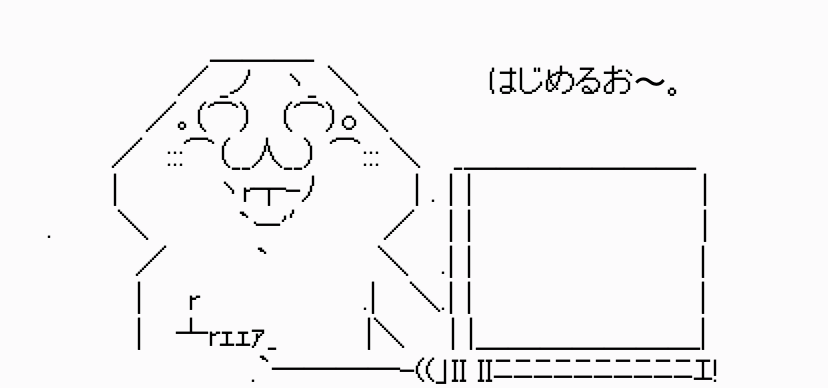
\includegraphics[width=1.0\maxwidth]{./images/00-preface/greetings04.png}%
\label{image:00-preface:greetings04}
\end{reviewimage}
